\ifdefined\THESIS
    \chapter{\uppercase {Data Collection}}

\else
    \section{Data Collection}
\fi

\section{Definitions}

Before going into the details of the data collection, we first define a few
terms to simplify the process of explaining how the data was collected.
%
Figure~\ref{fig:Terms} shows a social graph and uses most of the terms defined
in this section.
%
\textbf{Contacts} are defined to be the set of a user's friends, followers, and
people who a user mentioned in her tweets (i.e., people the user speaks to).
%
Since Twitter does not provide a mechanism to determine who mentioned a given
user, only one-directional conversation is considered.
%
In some blogging platforms, such as Tumblr, it is relatively easy to find the
communication edges that point back toward a user.
%
In those platforms, it would be fairly straightforward to use that information
in location prediction.

\begin{figure}[tbh]
\centering
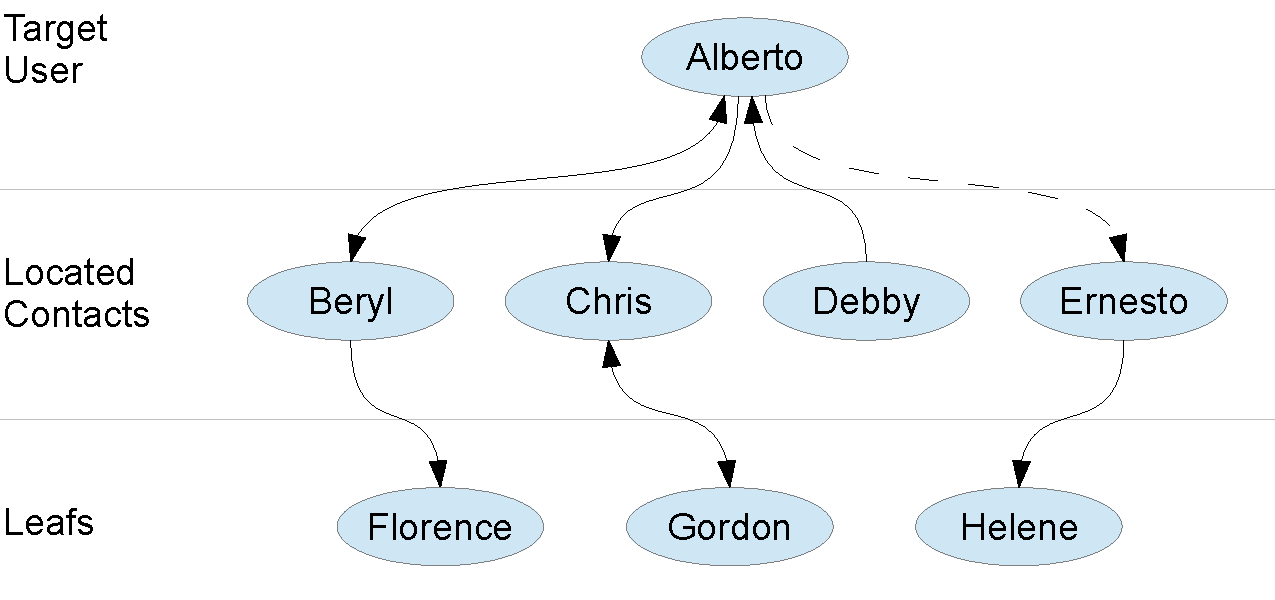
\includegraphics[width=\linewidth]{figures/terms.pdf}
\caption{
A small sample social graph for illustrating definitions used in this paper.
Alberto adds location information to his tweets.
Beryl is a reciprocal friend of Alberto, Chris is just a friend since Alberto
follows Chris, Debby is just a follower, and Ernesto is just mentioned.
The line to Ernesto is dashed to show that there is no friend/follow
relationship between Alberto and Ernesto.
The other arrows show who follows whom.
}
\label{fig:Terms}
\end{figure}

Any given contact can be categorized into precisely one of these four disjoint
sets:
\begin{description}
\item[reciprocal friend] The target user follows this user and is followed
    back.
\item[just friend] The target user follows this user and is not followed
    back.
\item[just follower] The target user is followed by this user, but does
    not follow them.
\item[just mentioned] The users do not follow each other, but the target
    user mentioned the name of the other user in a tweet.
\end{description}

Our crawler starts from a set of seed users and goes two steps out on the
social graph.
%
We created labels for the seed users and each of the steps along the way:

\begin{description}
\item[geo-located users] These users choose to use Twitter's location sharing
    features, which means that we have precise latitude and longitude
    coordinates for their location.
\item[\emph{needs a name}] \emph{geo-located users for understanding geo-coding}
\item[target users] These are a randomly chosen subset of the geo-loacted users
    who have at least one contact.
\item[located contacts] These are the 25 randomly chosen contacts of
    target users who have locations that we can decode.
\item[leaves] These are at most 100 of the contacts of the located contacts.
    When we selected leaves, we excluded the target users from the contacts so
    that the distances to contacts would be independent from the distances to
    leaves.
\end{description}

\emph{neighbors vs located contacts}


\section{Data Collection}
To investigate how social relation and geographical distance between the
relations correlate, we sample a dataset from Twitter.
%
Our analysis and prediction is based on data collected from Twitter during
May, June, and July of 2012.

We built a crawler to find these contacts for users who used Twitter's Location
Feature to disclose their location.
The crawler sampled over one hundred million geo-coded tweets by monitoring
Twitter's public streaming API for all of May 2012.
% 118,464,320 lines including keepalive newlines and non-status messages.
In the dataset, users are filtered who have strict privacy settings, have
neither friends nor followers, or posted fewer than three tweets in the sampled
dataset.
For each user with geo-coded tweets, we use the median latitude and median
longitude of the locations of the user's tweets as an approximation of her home
location.
Some Twitter accounts, such as accounts that posted jobs, would
move around faster than a human could possibly move.
To account for this, the crawler calculated the distance between each tweet and
the user's home location.
The crawler ignored users if the median distance from their tweets to their
home location was greater than 50 miles.
This left us with 1,695,784 geo-located users.
To enable parallelization, we divided those users into 100 groups based on
the two least significant digits in their Twitter user id, and randomly selected
2500 users from each of the groups.
%
This gave us the 250,000 target users that we planned to use for our
analysis and experimentation.
%
After crawling these users' friends and followers, we found 416 users who did
not have any neighbors with a location field that we could parse.
%
We filtered them out and used the remaining 249,584 for analysis and
experimentation.


\emph{How many contacts per target user?}

For all of the target users, the crawler used Twitter's API to download
the users' 100 most recent tweets, a list of friend ids, and a list of follower ids.
The crawler also downloaded the profiles for up to 100 friends, followers, and
people they mention in their tweets.
%
If they had over 100 in total, it chose a random sample of 100 profiles that
included at most 25 of each of the four types of contacts defined previously:
reciprocal friends, just friends, just followers, and just mentioned.
%
From that 100, we picked at most 25 contacts with locations we could decode to
be the located contacts. For those located contacts, we downloaded their
friends, followers, and tweets.
%
We finished this process by downloading 100 profiles of the contacts of the
contacts.
%
Since the Twitter social network graph has a large strongly connected
component, there are a significant number of users who are contacts or leafs for
more than one target user.
%
In the end, we collected just over 73 million Twitter user profiles.

%\begin{table}[tbh]
%\centering
%\begin{tabular}{l r l}
%    Data Set & Size & Description \\
%    \hline
%    % 249,584
%    Target 250 thousand & A randomly selected subset of
%    the geolocated users used for generating all the figures in
%    section~\ref{sec:analysis} and   \\
%    % 894,617
%    Geocoding Training & 895 thousand & geo-located users who where not
%    target but who did fill out the location field of their profile
%    \emph{this data set needs a better name}\\
%    % 10,081,957
%    Contacts & 10 million & Friends, followers, and mentions of the target
%    users \\
%    % 71,596,805 minus some of 250k
%    Leafs & 71 million & The contacts of the contacts \\
%\end{tabular}
%\label{tab:DataTypes}
%\caption{\emph{I'm not convinced this is a good way to do show the datasets.
%Should we merege this into the bulleted list in the previous subsection?}}
%\end{table}

\section{Geocoding}
We used Gisgraphy\footnote{\url{http://www.gisgraphy.com/}} to do geocoding.
%
Gisgraphy does full-text search on the
GeoNames\footnote{\url{http://www.geonames.org/}} database using Lucene.
%
Since it runs locally it is not limited to a certain number of queries per day.
%
Gisgraphy's geocoder returns ranked results based on a full text search
over millions of geographical features such as countries, cities, and schools.

The location field on a user's profile is just a text field that asks the user
to respond to ``Where in the world are you?''.
%
Responses vary from precise latitude and longitude coordinates entered
automatically by smartphone apps to jokes and nonsense.
%
Our system does some preprocessing before sending user-submitted locations to
the geocoder.
%
First, it uses a regular expression to find latitude and longitude coordinates,
which are treated as if they were a unique type of location returned by the
geocoder.
%
Occasionally, users would put two locations separated by a slash, dash or a
conjunction, and we pick the first one that we could decode.
%
If the geocoder did not return any results for a user, our system tried to
geocode both locations and returned the first location that the geocoder
understood.

Some locations are significantly more useful than others.
For example, even though Rhode Island and Montana are both states with around
one million people, Rhode Island is smaller, and as a result, much more useful
in estimating the location of a user.
To make the results of the geocoder more useful, we devised a method to
estimate the accuracy of a location returned by the geocoder.

\begin{table}[tb]
\centering
\caption{Example Median Location Errors (in miles).}
\begin{tabular}{l r r}
Location&Number of Users&Median Error\\ \hline
``Bronx''&438&4\\
``New York''&7483&175\\
``Pluto''&238&8272\\ \hline
\\
Place Type&Number of Users&Median Error\\ \hline
(latitude, longitude)&76552&3\\
A City&20914&6\\
A Hotel&1052&29\\
An Airport&410&258\\
A Stream&739&2373\\
\hline\end{tabular}
\label{tab:MedianLocErr}
\end{table}

Since we only selected 250,000 of the 1,695,784 users who posted tweets with
location information for location prediction and analysis, the remaining users
could be used for evaluating the geocoder.
%
894,617 of the users who posted geo-located tweets also filled in the
the free-response location field with something that the geocoder was able to
decode.
%
We can compare the results of the geocoder to the location of the geo-located
tweets for these users to quantify how accurate the geocoder is for certain
types of locations.


We define the \textbf{location error} to be the great circle distance between a
user's home location and the location returned from the geocoder.
%\[
%LE = |l^h - l^g|
%\]
%
The location error for a user can vary from less than a mile to over ten
thousand miles.
%
We calculated the location error for each of the geo-located users selected for
evaluating the geocoder, and sorted the users by their location.
%
For the 17,370 locations that had at least three users, we calculated the median
location error for that location.
%
All the users who were at locations with only one or two users were grouped
according to the type of location returned by the geocoder.
%
We calculated the median error for each location type.
%
The median is more appropriate than the average or standard deviation because
those metrics are strongly affected by large outliers.
%
We choose to make the cutoff three because that is the smallest value where the
median is not just an average.
Table~\ref{tab:MedianLocErr} shows the median location error for a few example
locations and location types.

\emph{work in progress ahead}

We treat each location returned by the geocoder as a tuple $(l^g_i,p_i,t_i)$,
where $l^g_i$ is the latitude and longitude, $p_i$ is the id of the place, and
$t_i$ is the id of the type of place.

\emph{Can I express PLE in math?}

This gives us a method to estimate the quality of a coordinate returned by
Gisgraphy.
%
We define the \textbf{predicted location error (PLE)} for a given location to
be the median location error if it is one of the 17,370 locations that had
at least three users; otherwise, it is the median location error for the location's
type.
%
For example, one user had ``PDX,OR'' in his location field.
%
Gisgraphy identifies this as ``Portland International Airport''.
%
Since it is not one of the most common locations, its PLE is determined by its
place type to be 258 miles as seen in Table~\ref{tab:MedianLocErr}.
%
An airport is a bad location name since airports tend to have regional names
and people who report their location as an airport are likely to move around a
lot.

\begin{figure}[tb]
\centering
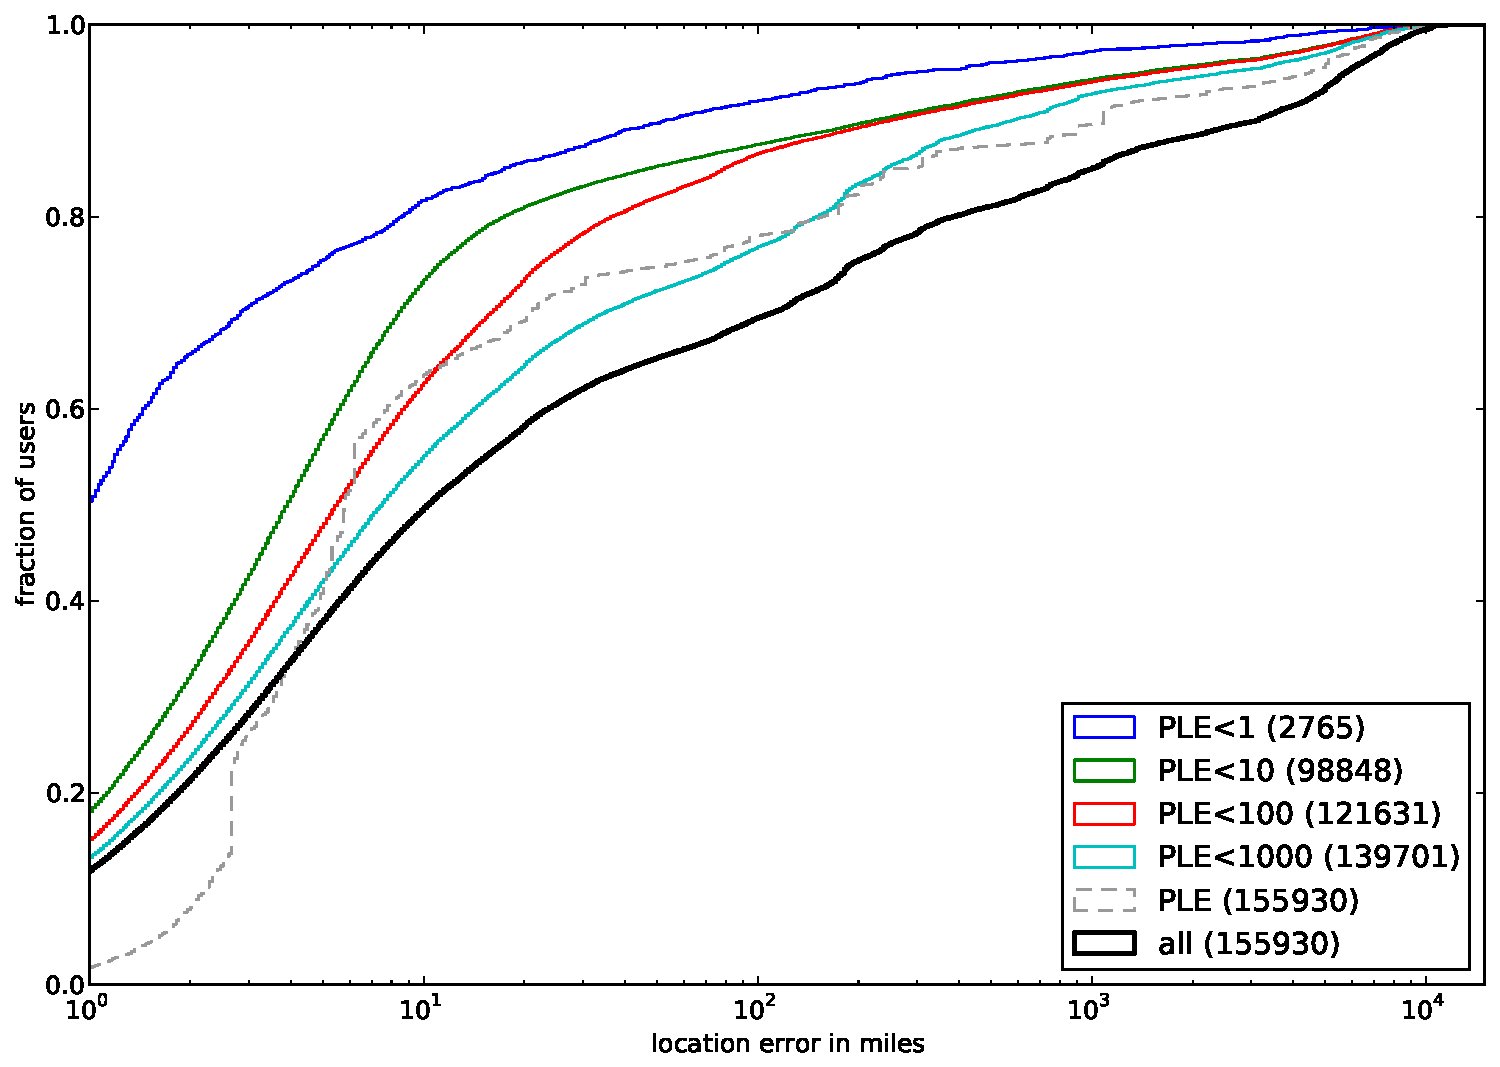
\includegraphics[width=\linewidth]{figures/mloc_mdist.pdf}
\caption{
Cumulative distribution function(CDF) of the distance between geo-located
users' tweets and their geocoded self-reported location.
%
The distances are split into bins based on the predicted location error(PLE).
%
The blue lines show that locations with a low PLE tend to be accurate, and
locations with a high PLE are rarely accurate.
%
The dotted line shows the values of the PLE for all the
users in this graph.
%
63\% of these users have a PLE less than 10 miles.
}
\label{fig:DiffMlocMdist}
\end{figure}

Figure~\ref{fig:DiffMlocMdist} shows the result of using the PLE to ignore
users who have low quality locations such as ``Pluto''.
The solid black line represents the normal results of geocoding where the
location error is less than 1000 miles for 85\% of the users.
The cyan line shows the results of removing locations with a PLE greater than
or equal to 1000 miles.
After removing only 10\% of the users, 93\% of them are within 1000 miles.
\emph{What?}
